
%%%%%%%%%%%%%%%%%%%%%%% xxxxxxxxxxxxxxxx %%%%%%%%%%%%%%%%%%%%%%%%%
%
%	copyright by Springer Heidelberg
%   http://www.springer.com/lncs       Springer Heidelberg 2006/05/04
%
%
%%%%%%%%%%%%%%%%%%%%%%%%%%%%%%%%%%%%%%%%%%%%%%%%%%%%%%%%%%%%%%%%%%%


\documentclass[runningheads,a4paper]{llncs}

\usepackage{amssymb}
\setcounter{tocdepth}{3}
\usepackage{graphicx}
\usepackage{caption}
\usepackage{url} %takes care of proper line breaks for URLs
\usepackage{hyperref} % creates clickable links and references.
\usepackage{subcaption}
\usepackage{float}% exact position of figures
\usepackage[backend=biber]{biblatex}
\usepackage{listings}
%\usepackage[T1]{fontenc}
\bibliography{citations}

\setlength{\parindent}{0pt} % no indent on new paragraphs

\newtheorem{defn}{Definition}


\begin{document}

\mainmatter  % start of an individual contribution

% first the title is needed
\title{Domain Specific Modeling}

% a short form should be given in case it is too long for the running head
\titlerunning{Domain Specific Modeling}


\author{Tim Schneider\\ tim-1.schneider@uni-ulm.de}
\institute{Institute of Databases and
Information Systems, Ulm University}


\maketitle


\begin{abstract}
%The abstract should summarize the contents of the paper and should
%contain at least 70 and at most 150 words. It should be written using the
For centuries people from da Vinci to Einstein have created models to help them better 
understand patterns and processes in the world around them. 
Domain-specific modeling languages enable users with few or even no programming skills to implement their own models.
This paper gives a  brief overview over different domain-specific modeling languages that enables these users 
to implement their own models without extensive knowledge in general purpose programming languages (e.g. C++, Java, ...).
Additionally, some tools for creating textual and graphical modeling languages are presented, which allow 
creating new domain-specific modeling languages without requiring knowledge in parser-construction or 
skills in programming a graphical model editor.
\end{abstract}

\section{Introduction}
Computers and smartphones have become an integral part of our everyday life, 
making software development becoming increasingly important over the last years.
As software development projects are getting bigger and more complex it is desirable to  
support domain experts using their knowledge for implementing IT systems.
Most domain experts have few or even no programming skills at all, which requires them to engage specialists to
create software based on their description. 
In traditional software development these specialists include project-leaders, analysts and developers that need 
to communicate with each other to implement features based on domain experts descriptions. 
This communication overhead can be time-consuming and error prone as the involved stakeholders
create their very own abstractions when dealing with these descriptions during the software development process.
As a result the created software may not correspond to the domain experts intents.
Fig. \ref{fig:swingexample} illustrates how the domain experts description is perceived by the different stakeholders:
Ideas, described by a domain expert, are percieved by a project-leader in a biased way, removing details that are perceived not relevant for the solution
of the described problem. Often, the decision if a detail (e.g. additional swing seats) is relevant for the solution is made unconsciously. 
A project leader communicates the perceived information to an analyst, who build his own abstraction of the problem by adding or removing other details
that are percieved relevant. So does a programmer who implements the software. As a result, the implemented software may not be what the end-user really needed.
\begin{figure}[h]
\begin{center}
\begin{tabular}{|c|c|c|c|c|}\hline
&&&&\\
\begin{subfigure}[t]{0.15\textwidth}\centering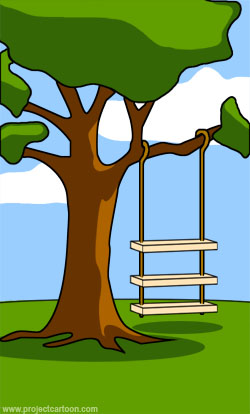
\includegraphics[width=0.9\columnwidth]{images/howexplained}
\caption*{\tiny \centering How the domain expert explained it}\label{fig:howexplained}\end{subfigure}&
\begin{subfigure}[t]{0.15\textwidth}\centering
\includegraphics[width=0.9\columnwidth]{images/howunderstood}
\caption*{\tiny \centering How the project-leader understood it}\label{fig:howunderstood}\end{subfigure}&
\begin{subfigure}[t]{0.15\textwidth}\centering
\includegraphics[width=0.9\columnwidth]{images/howdesigned}
\caption*{\tiny \centering How the analyst designed it}\label{fig:howdesigned}\end{subfigure}&
\begin{subfigure}[t]{0.15\textwidth}\centering
\includegraphics[width=0.9\columnwidth]{images/howprogrammed}
\caption*{\tiny \centering How the programmer wrote it}\label{fig:howprogrammed}\end{subfigure}&
%\begin{subfigure}{0.2\textwidth}\centering
\includegraphics[width=0.8\columnwidth]{images/howdocumented}
%\caption{How it was documented}\label{fig:howdocumented}\end{subfigure}\\
%\begin{subfigure}{0.2\textwidth}\centering
\includegraphics[width=0.85\columnwidth]{images/howinstalled}
%\caption*{\centering  What operations installed}\label{fig:howinstalled}\end{subfigure}&
%\begin{subfigure}{0.2\textwidth}\centering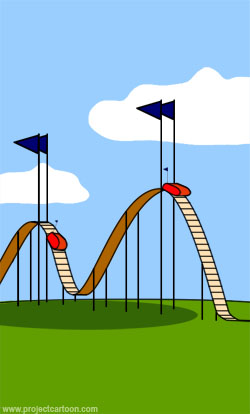
\includegraphics[width=0.8\columnwidth]{images/howbilled}
%\caption{How the customer was billed}\label{fig:howbilled}\end{subfigure}&
%\begin{subfigure}{0.2\textwidth}\centering
\includegraphics[width=0.85\columnwidth]{images/howsupported}
%\caption*{\centering How it was supported\newline}\label{fig:howsupported}\end{subfigure}&
%\begin{subfigure}[t]{0.15\textwidth}\centering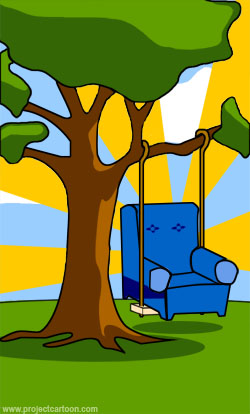
\includegraphics[width=0.9\columnwidth]{images/howdescribed}
%\caption*{\tiny \centering How it was promoted}\label{fig:howsupported}\end{subfigure}&
%\begin{subfigure}{0.2\textwidth}\centering
\includegraphics[width=0.85\columnwidth]{images/whendelivered}
%\caption*{\centering  When it was delivered\newline}\label{fig:whendelivered}\end{subfigure}\\
\begin{subfigure}[t]{0.15\textwidth}\centering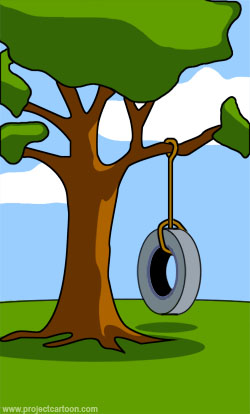
\includegraphics[width=0.9\columnwidth]{images/whatneeded}
\caption*{\tiny \centering What the user really needed}\label{fig:whatneeded}\end{subfigure}\\
\hline
\end{tabular}
\caption{Biased perception of information in the software development process, based on different mental models. [images from \cite{projectcartoon}]}
\label{fig:swingexample}
\end{center}
\end{figure}
To avoid errors originating from the biased perception of information by the different stakeholders (i.e. end-user, project-leader, analyst, developer), 
it is desirable to enable domain-experts to implement their own ideas.
General purpose programming languages, on the other hand, can be hard to learn for people without programming skills.
Domain-specific modeling offers an approach to ease the need to learn a general purpose programming
by creating \emph{models} (Def. \ref{def:model}) with \emph{domain-specific modeling languages} (Def. \ref{def:dsml})
using using terms and concepts that are well understand by domain experts.
Therefore this paper gives a brief introduction into the fundamentals of domain-specific modeling languages and presents
different  modeling languages languages, which allow domain-experts with few or no programming skills to implement their own models.
Additionally, the tools Xtext and GMF are persented, which allow the creation of different kinds of domain-specific modeling languages
based on a kind of meta-model utilizing the Eclipse Modeling Framework (EMF).

% \begin{itemize}
%  \item can help experts and novices builing Models for different domains
%  \item enables novices with few or even no programming skills at all to implement their own models (e.g. MindStorm,Starlogo)
%  \item supports domain experts by setting focus on the domain-specific problems (e.g. SimuLink,BPMN)
%   \end{itemize}

\section{Fundamentals}
\label{section:fundamentals}
This section gives a brief overview over the fundamentals of domain-specific modeling languages 
and the terms used in the following sections. This includes Definitions of the terms \emph{model} (Def. \ref{def:model}), 
\emph{domain} (Def. \ref{def:domain}) and \emph{domain-specific modeling languages} (Def. \ref{def:dsml}).

\begin{defn}
    \label{def:model}
    A \underline{model} is a formal representation of entities and relationships in the real world (abstraction) 
    with a certain correspondence (homomorphism) for a certain purpose (pragmatics) \cite{stachowiak1973allgemeine}.
\end{defn}
This definition contains three aspects: abstraction, homomorphism and pragmatics.
A model should create a simplified view on the represented entities and relationships and 
only contain details, which are relevant for a given application scenario (abstraction).
Additionally statements on the model elements should hold for the represented entities and relationships (homomorphism).
The question, which details are relevant and therefore should be included in the model is determined by the purpose of a model (pragmatics).  
\\\\
Creating models is something we do in our everyday lives:
When building a house using LEGO blocks a child creates a model which serves as a representation for a building in the real world.
It is a simplified view on the original as it abstracts from details, like used materials, installed cables and water pipes and focuses
on the shapes of the building. Another example for creating models is an architect, who creates blueprints for a house, serving as a model for it.
Blueprints contain 2D projections of walls and installations from different viewpoints and abstract from the original by omitting
details like materials and some 3D information. As one can see from these examples, these abstractions also contain a representational bias:
Electric cable installations and water pipes cannot be expressed with LEGO but can with blueprints.
LEGO models, on the other hand, allows to model 3D structures while blueprints cannot.
In this example, the child and the architect have different views on the same thing (houses), but share a common understanding the real world.
Despite their different level of expertise, both the child and the architect know that the concepts \textit{wall} and \textit{roof} 
are related to parts of a building and that a house needs both to be a valid house.
Based on this examples one can define the term \textit{domain} as follows:
\begin{defn}
\label{def:domain}
A \underline{domain} is the common knowledge of the requirements, concepts and functionality in a field of application.
\end{defn}
Based on Def.\ref{def:model} and Def.\ref{def:domain} one can define the term \emph{domain-specific modeling language} as follows:
\begin{defn}
\label{def:dsml}
A \underline{domain-specific modeling language} is a textual or graphical representation of the concepts, entities and relationships that are 
relevant for a specific domain.
\end{defn}
One can distinguish two types of domain-specific modeling language modeling languages:
While \emph{textual modeling languages} use textual descriptions to represent entities and relationships from the real world,
\emph{graphical modeling languages} use graphical shapes, lines and arrows for the same purpose.
The same model may be expressed in both, a graphical or textual modeling languages.
For example: A finite state machine can be represented as a set of nodes, labeled boxes and arrows, while it can also be 
represented by a textual description following a grammar to represent the same finite state machine as seen in Fig. \ref{compare:textgraphiclang}.
\begin{figure}[H]
      \centering
      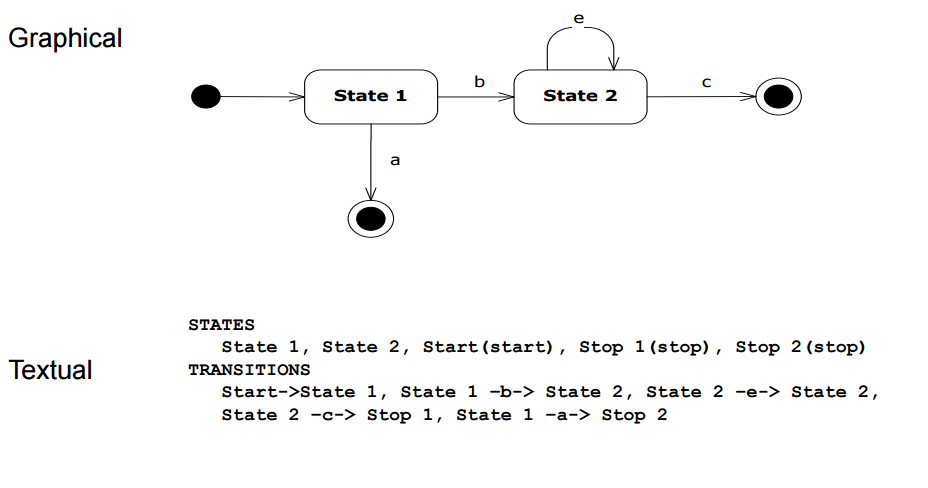
\includegraphics[width=.8\textwidth]{images/GraficalTextualComparison.PNG}
      \captionof{figure}{Comparison between textual modeling language and graphical modeling language for the same model of a finite state machine.}
      \label{compare:textgraphiclang}
\end{figure}
The decision whether a graphical modeling language or textual modeling language is chosen for the implementation of a modeling tool 
may also be influenced by the targeted audience: A software-developer has a deep knowledge in using text-based editors, while 
children may not have these kind of expertise and therefore prefer a more graphical representation. 
Different levels of expertise can also be observed with regards to domain knowledge:
A software-developer probably has a more detailed knowledge in the computer science domain compared to a medical doctor.


 \section{Domain-Specific Modeling Languages}
 \label{section:dsml}
 As there is a variety of software tools available, which implement different modeling languages, this section will give an overview 
 about modeling languages designed to support users with few or even no programming languages in creating models and help them better 
 understand patterns and processes in the world around them.
 
 \subsection{StarLogo TNG}
  %enable students to build simulations and learn features of complex systems without extensive background knowledge (Klopfer et al., 2009a; 2009b)
  %provides an environment for building agent-based models
  StarLogo is a client based modeling software, developed specifically to enable students to 
  create models for the simulation of complex systems without extensive programming skills \cite{klopfer2009starlogo}.
  It provides a graphical modeling language using blocks instead of a textual syntax. 
  These blocks are coloured based on the function they have in the program and their shapes only allow syntactically correct constructs \cite{klopfer2009starlogo}.
  This eases the learning of basic programming concepts such as control-flow (e.g. loops, if-then statements),
  assignments and methods by providing intuitive graphical mappings. Since StarLogo TNG uses these puzzle-piece shapes, understanding 
  control-flow, for example, ``requires little more than visually parsing the \texttt{if} or \texttt{repeat} commands 
  to conclude that items placed within the then slot will be performed if the items placed within the 
  test slot are true, or the items placed within the do slot will be subject to the number of repetitions placed within the times slot''\cite{smith2011biology}.
  Using puzzle-piece shapes for basic programming concept avoids syntactic errors, 
  which are one of the main difficulties in learning textual programming languages.
  Figure \ref{fig1} shows an exmaple for the blocks used by StarLogo TNG: 
  the curved shape of a Boolean variable is easy to distinguish from the pointed shape of a number value.
  
  \begin{figure}[H]
	\centering
  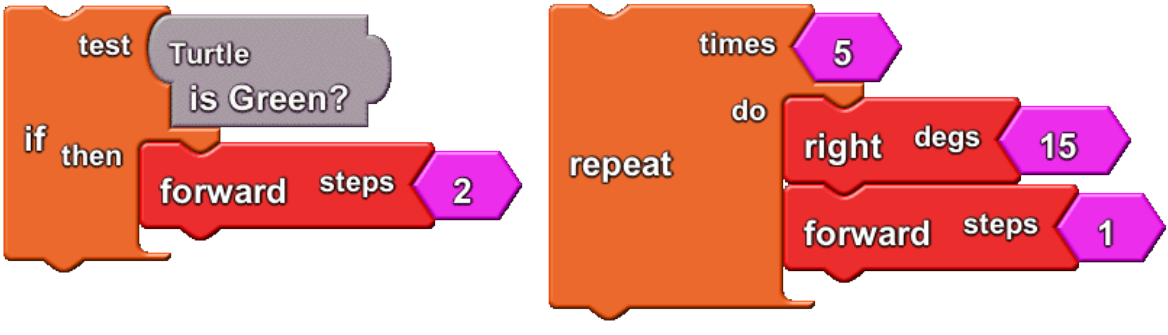
\includegraphics[width=0.5\textwidth]{images/StarLogoTNGBlocksEx.PNG}
	\caption{ StarLogo TNG’s graphical programming blocks. Example: \texttt{if} (left) and \texttt{repeat} (right) blocks are shown. The
	  if block commands a Turtle agent to take two steps forward if it is green; the repeat block commands an agent to
	  repeat five times the sequence of turning right 15 degrees and taking one step forward. [images from \cite{smith2011biology}]}
	\label{fig1}
  \end{figure}
  
  %   \begin{itemize}
%   \item is a client-based modeling and simulation software
%   \item enables secondary school students and teachers to model decentralized systems through agent-based programming
%   \item facilitates the creation and understanding of simulations of complex systems
%   \item graphical programming blocks instead of text-based computer code
%   \end{itemize}

   \subsection{Scratch}
  Scratch is graphical modeling languages for visual programming that allows users (primarily ages 8 to 16 \cite{maloney2010scratch}) to learn
  computer programming while working on personally meaningful projects such as animated stories and games. 
  A major design goal of Scratch is to support self-directed learning through tinkering and collaboration with peers \cite{maloney2010scratch}. 
  Scratch uses blocks (Fig.\ref{subfig:highlightconcepts}) similiar to StarLogo TNG for creating models. One of the key features of Scratch is that it is always \emph{live},
  which means that there is no compilation step or edit/run mode distinction. A user can see what a command or program fragment does by clicking 
  it at any time. This also implies that a user can change parameters or add new blocks to a script while it is running.
  Because it is live, Scratch encourages users to experiment with it and supports
  a bottom-up approach to writing scripts where small chunks of program fragments are assembled and tested, then combined into larger units.
  Additionally, Scratch provides visual feedback to show script execution by surrounding a script with a white border when it is 
  running (Fig. \ref{subfig:blocktest}). This feedback
  helps the user understand when scripts are triggered and how long they run. If an error is encountered then the border of the 
  affected script turns red and the block that caused the error is highlighted in red. 
  Furthermore Scratch eliminates the need for syntax error messages by using 
  puzzle-piece shapes which only fit where it makes sense. Additionally, Scratch tries to avoid runtime errors by making all blocks be
  \textit{failsoft}. ``Rather than failing with an error message, every block attempts to do something sensible even when presented with out-of-range inputs''\cite{maloney2010scratch}.
  Even though eliminating the runtime error messages does not eliminate the errors, by following this approach, a script can always be tested by the user.
  %Since a program that can be tested even if the result is incorrect, it is favoured to not be able to run or compile it at all.
% \begin{figure}[h]
% \begin{center}
% \begin{tabular}{|c|c|}\hline
% &\\
% \begin{subfigure}[t]{0.45\textwidth}\centering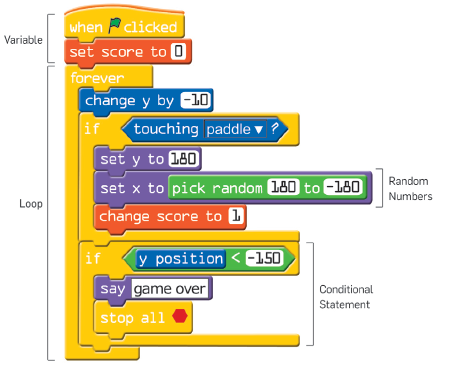
\includegraphics[width=0.9\columnwidth]{images/Snatch1.PNG}
% \caption*{\tiny \centering How the customer explained it}\label{fig:howexplained}\end{subfigure}&
% \begin{subfigure}[t]{0.45\textwidth}\centering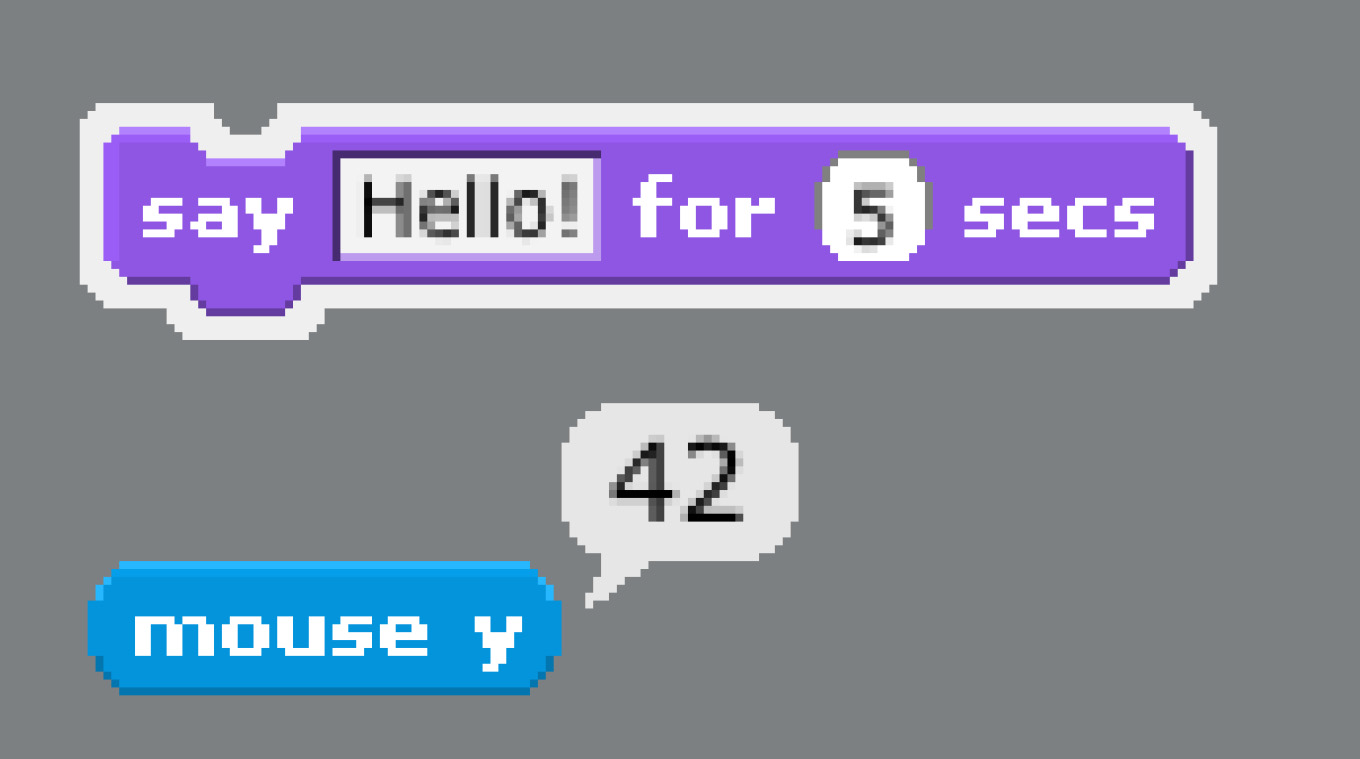
\includegraphics[width=0.9\columnwidth]{images/ScratchLive.png}
% \caption*{\tiny \centering How the project-leader understood it}\label{fig:howunderstood}\end{subfigure}\\
% \hline
% \end{tabular}
% \caption{Communication chain in the software development process with different mental models.}
% \label{fig:swingexample}
% \end{center}
% \end{figure}

\begin{figure}[ht]
\centering
\begin{subfigure}[t]{0.45\textwidth}\centering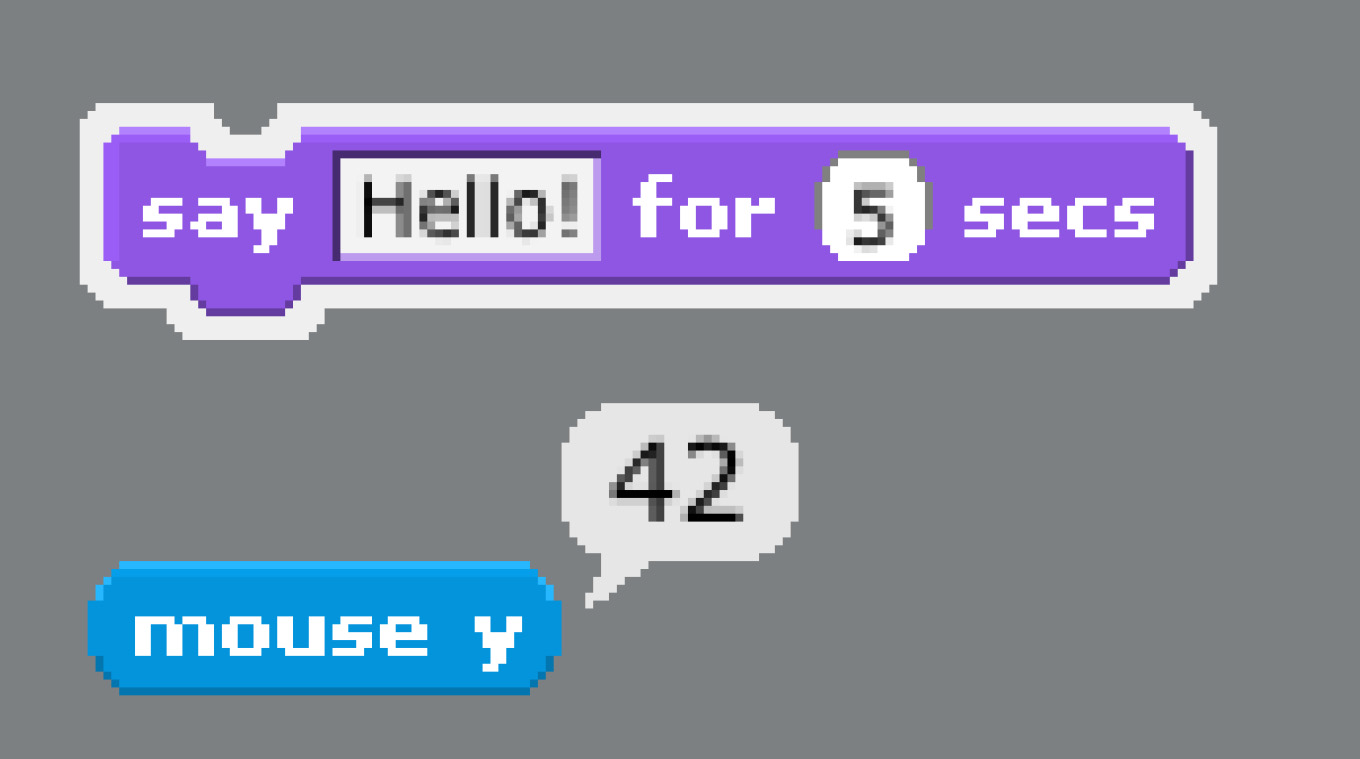
\includegraphics[width=0.9\columnwidth]{images/ScratchLive.png}
\caption{Blocks can be tested simply by clicking on them. A white border indicates that a block or 
stack is running. Function blocks show their output in a  bubble.}\label{subfig:blocktest}\end{subfigure}
\hspace*{\fill}
\begin{subfigure}[t]{0.45\textwidth}\centering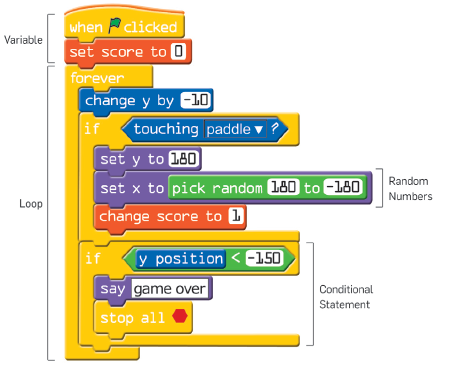
\includegraphics[width=0.9\columnwidth]{images/Snatch1.PNG}
\caption{Sample Scratch script (from Pong-like paddle game) highlighting computational and mathematical concepts.}\label{subfig:highlightconcepts}\end{subfigure}
\begin{subfigure}[t]{0.9\textwidth}\vspace{1cm}\centering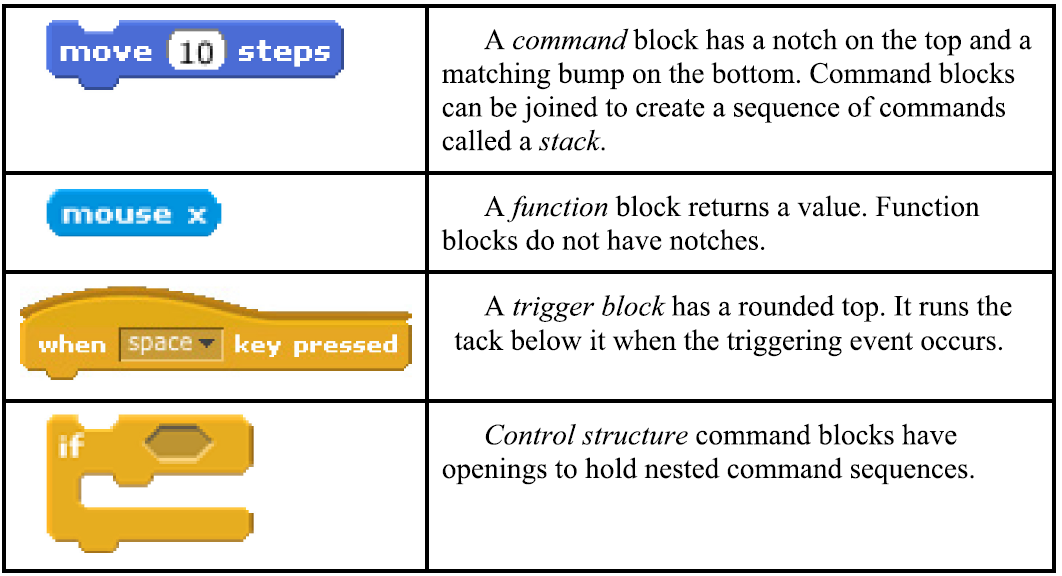
\includegraphics[width=0.9\columnwidth]{images/ScratchBlockTypes.PNG}
\caption{Scratch block types.}\end{subfigure}
\caption{Concepts in Scratch for supporting users with programming. [images from \cite{maloney2010scratch}]}
\end{figure}

  \subsection{PhyDSL}
  \label{subsection:PhyDSL}
  Both StarLogo and Scratch use graphical modeling languages for creating models. 
  \emph{PhyDSL} is a tool, designed as an Eclipse plugin that uses a textual modeling language for creating models for the game development domain.
  It was designed for the purpose of supporting the fast prototyping of physics-based games, including platform, shoot-em-up, 
  puzzle and maze games \cite{guana2014phydsl}. 
  The provided frontend includes a text editor (including syntax highlighting and text completion), which is used to define gameplay in highlevel
  terms describing the gameplay static, dynamic elements and their behaviors by a domain-specific modeling language.  
  It is based on the \emph{Eclipse Modeling Framework} \cite{gronback2009eclipse} (EMF) and uses codegeneration for deriving C\# code supported by Microsoft’s
  DirectX API. 
  The modeling language provided by PhyDSL consists of four gameplay definition sections: mobile and
  static actor definition (Fig. \ref{actordef}), 
  environment and layout definition (Fig. \ref{envdef}), 
  activities definition (Fig. \ref{activitiesdef}), 
  and scoring rules definition (Fig. \ref{rulesdef}).
  
%  \begin{itemize}
%   \item textual modeling for (simple) game dev domain
%   \item based on EMF
%   \item allows codegeneration from the created models
%   \item mobile gameplay definition sections:
%     \begin{itemize}
%     \item static actor definition
%     \item environment and layout definition
%     \item activities definition
%     \item scoring rules definition
%     \end{itemize}
%   
%   \end{itemize}
\begin{figure}[H]
\centering
\begin{subfigure}[t]{0.45\textwidth}\centering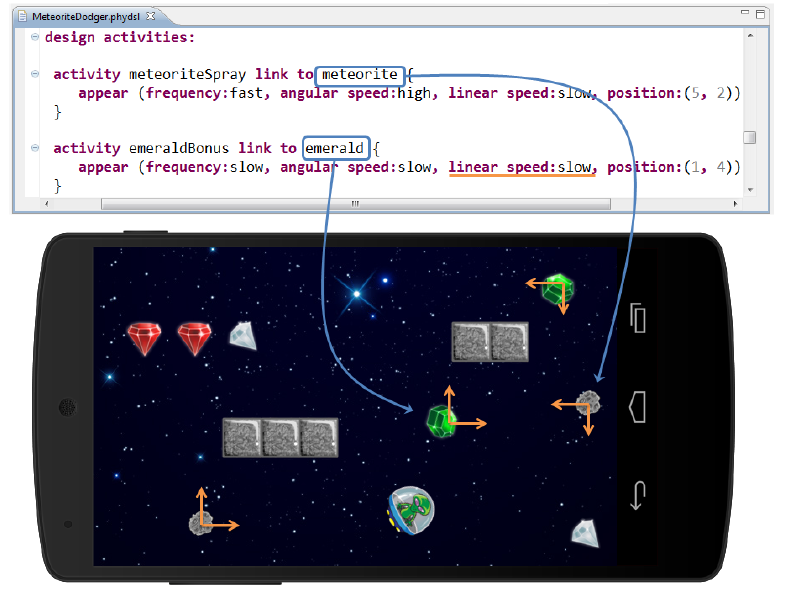
\includegraphics[width=.9\columnwidth]{images/PhyDSL3.PNG}
\caption{Activities Definition}\label{activitiesdef}\end{subfigure}\hspace*{\fill}
\begin{subfigure}[t]{0.45\textwidth}\centering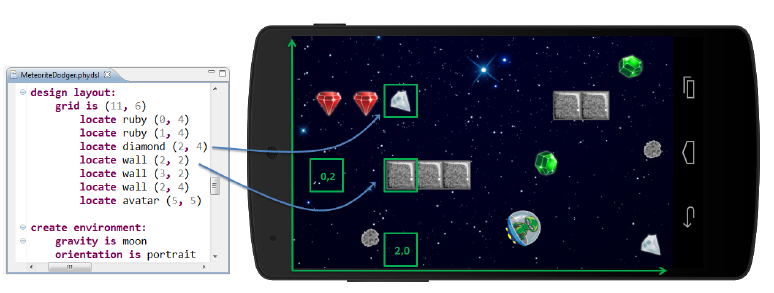
\includegraphics[width=.9\columnwidth]{images/PhyDSL2.PNG}
\caption{Environment and Layout Definition}\label{envdef}\end{subfigure}
\begin{subfigure}[t]{0.45\textwidth}\centering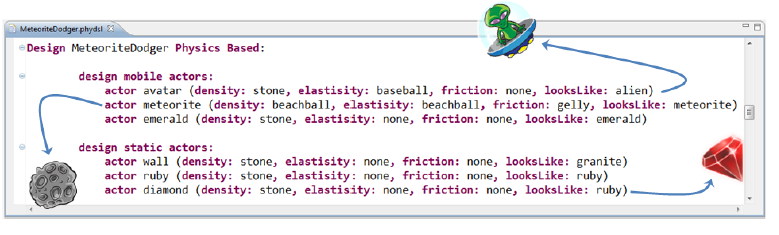
\includegraphics[width=.9\columnwidth]{images/PhyDSL1.PNG}
\caption{Static Actor Definition}\label{actordef}\end{subfigure}\hspace*{\fill}
\begin{subfigure}[t]{0.45\textwidth}\centering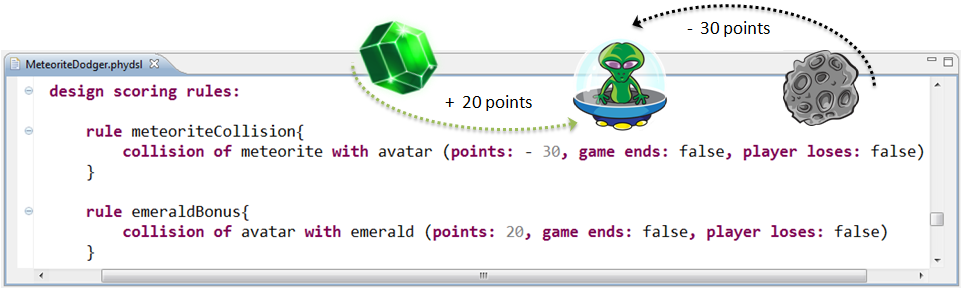
\includegraphics[width=.9\columnwidth]{images/PhyDSL4.PNG}
\caption{Scoring Rule Definition for Collision Rules}\label{rulesdef}\end{subfigure}
\caption{Phydsl:  describing the gameplay static, dynamic elements and their behaviors. [images from  \cite{guana2014phydsl}]}
\end{figure}

   \subsection{LEGO Mindstorms}
   Another example for a graphical modeling language made for end-users is the EV3 Programmer App \ref{fig:ev3app}
   for LEGO Mindstorms which includes a block-based graphical modeling langue for creating programms
   for the LEGO MindStorm Robots. Programs are loaded and executed on a EV3 Programmable Brick (Fig. \ref{fig:ev3pbrick}), 
   which offers input and output connections for interaction with sensors and actuators.
   Different colors are used to indicate whether a blocks triggers some action (green; Fig. \ref{fig:actionblocks}), is used for flow control (orange; Fig. \ref{fig:flowblocks}),
   reads data from some input (e.g. color sensor)(yellow; Fig.\ref{fig:sensorblocks}) or trigger some data operation (e.g. read or write some variable) (red; Fig. \ref{fig:operationsblocks}).
   
%   \begin{itemize}
%   \item EV3 Programmer App or Computer Software for programming lego robots in a graphical syntax 
%   \item action blocks (green), flow blocks (orange), sensor blocks (yellow), data operation blocks (red), advanced blocks (dark blue)
%   \item programms are executed on the EV3 P-brick. 
%   %https://www.lego.com/en-us/mindstorms/learn-to-program
%   \end{itemize}
  \begin{figure}[H]
\centering
\begin{subfigure}[t]{0.45\textwidth}\centering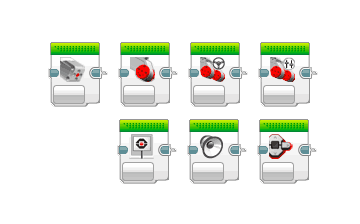
\includegraphics[width=.9\columnwidth]{images/LearnToProgram_action_blocks_landscape.png}
\caption{The action blocks control the actions of the program, e.g. motor rotations, image, sound and the light on the EV3 P-brick.}\label{fig:actionblocks}\end{subfigure}\hspace*{\fill}
\begin{subfigure}[t]{0.45\textwidth}\centering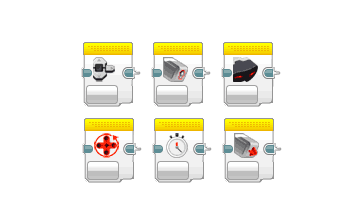
\includegraphics[width=.9\columnwidth]{images/LearnToProgram_sensor_blocks_landscape.png}
\caption{The sensor blocks allow to read the inputs, e.g. from a color sensor, IR sensor, touch sensor.} \label{fig:sensorblocks}\end{subfigure}
\begin{subfigure}[t]{0.45\textwidth}\centering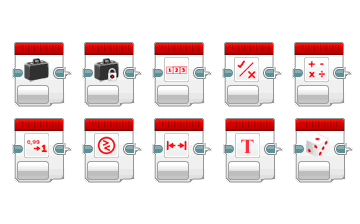
\includegraphics[width=.9\columnwidth]{images/LearnToProgram_operations_blocks_landscape.png}
\caption{The data operation blocks let the user write and read variables, compare values for example }\label{fig:operationsblocks}\end{subfigure}\hspace*{\fill}
\begin{subfigure}[t]{0.45\textwidth}\centering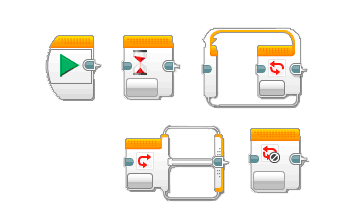
\includegraphics[width=.9\columnwidth]{images/LearnToProgram_flow_blocks_landscape.png}
\caption{The Flow blocks control the flow of the program.}\label{fig:flowblocks}\end{subfigure}
\caption{LEGO EV3 Programmer App: Different block types. [images from \cite{legoev3}]}
\end{figure}
  
\begin{figure}[H]
	  \centering
	  \begin{subfigure}[t]{0.45\textwidth}\centering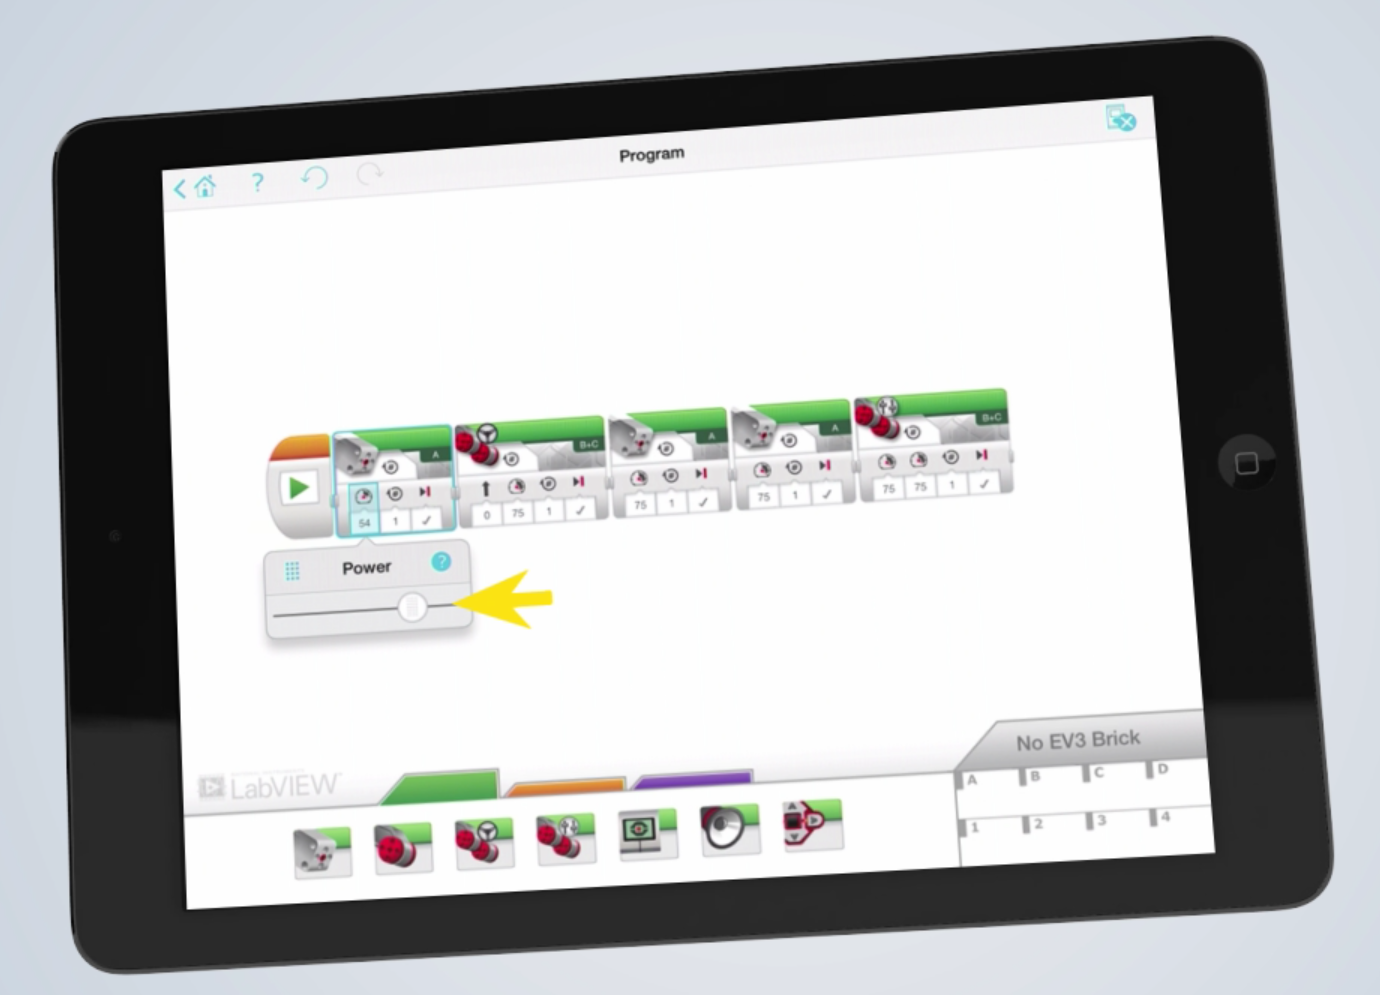
\includegraphics[width=.9\columnwidth]{images/mindstorms0.PNG}
	  \caption{EV3 Programmer App on a tablet used to create programms using a graphical modeling language. }\label{fig:ev3app}\end{subfigure}\hspace*{\fill}
	  \begin{subfigure}[t]{0.45\textwidth}\centering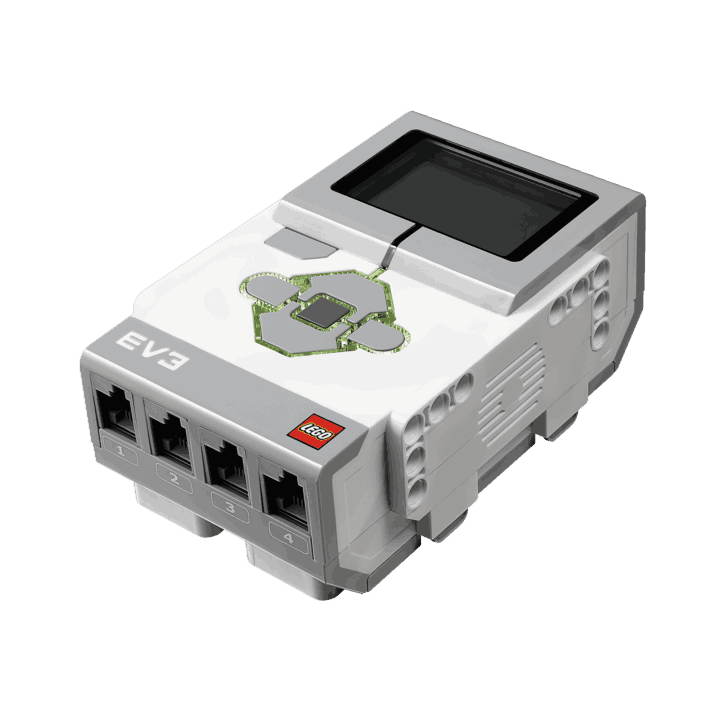
\includegraphics[width=.9\columnwidth]{images/ev3brick.png}
	  \caption{EV3 Programmable Brick with connections for different sensors and actuators. }  \label{fig:ev3pbrick}\end{subfigure}
	  \caption{EV3: Programming and execution are performed on different devices (Fig. \ref{fig:ev3app};\ref{fig:ev3pbrick}). [images from \cite{legoev3}]}
\end{figure}

    \section{Creating Domain-Specific Modeling Languages}
    \label{section:creatingdsmls}
    Domain-Specific Modeling Languages are implemented in various software tools using textual or graphical modeling languages.
    In fact, there are approaches to define these modeling languages as models using some kind of meta-language.
    Xtext and GMF are implementions for the Eclipse Modeling Framework (EMF), which adopt this approach.
    
    \subsection{Xtext}
    Xtext is a framework for development of programming languages and domain-specific modeling languages \cite{eysholdt2010xtext}.
    %It uses a syntax similar to extended backus-naur form (EBNF) to describe custom textual modeling languages.
    For this purpose, Xtext features a domain-specific modeling language, called \emph{Grammar Language}, designed for the description of textual modeling languages \cite{xtextgrammarlang}.
    To describe a custom modeling language, one has to define a grammar in a syntax similar to Extended Backus-Naur Form (EBNF).
    The Grammar Language contains terminal- and parser rules, used to generate a lexer and a parser.
    Terminal rules are used to transform the text input into a sequence of tokens, representing atomic symbols. This is performed during the lexing stage. 
    Afterwards, in the parsing stage, parser rules are applied to create a parse tree consisting of non-terminals and terminal tokens.
    Furthermore, parser rules are handled as kind of a building plan for the creation of a model.
    Different constructs like assignments or calls to other rules are used to fill the model with information from the text input. 
    Listing \ref{lst:fsmgrammar} contains a terminal rule called \texttt{ID}, matching a character sequence beginning with a 
    upper- or lowercase letter or underscore, followed sequence of alphanumeric values that is transformed to a token of the the type 
    \textit{ID}. Additionally, it shows how a FSM can be described by typing the string ``States:'' and a optional list of States, separated by commas,
    followed by the string ``Transitions:'' and a optional list of transitions, separated in the same way.
    The property \texttt{states}, which defines a composition of states, is composed by matching another parser rule \texttt{State} for states.
    The parser rule \texttt{State} creates a model element of the corresponding type at set the attribute id  to the value of the token with type \texttt{ID}. 
    The operator \texttt{?=} denotes that the attribute \texttt{isStart} is assigned to the Boolean value \textit{true} if the terminal \texttt{(start)} is matched afterwards. 
    From such a description in the Grammar Language, a custom text-editor for Eclipse is generated by Xtext. Furthermore, features of the generated text-editor include code-completion and syntax-highlighting
    as well as a parser for parsing models from text files specified in the defined grammar. This makes it easy for language design experts 
    to create models for custom modeling languages without requiring programming skills or knowledge on how to implement a parser.
    As the modeling language definitions are stored in the Ecore format \footnote{Ecore is a (meta-)model included in the Eclipse Modeling Framework (EMF), which is used to describe with elements, attributes and relationships are allowed 
    in a model. It is an implementation of the \emph{Meta Object Facility} (MOF) Standard \cite{mof20062}, specified by the OMG.}, other tools in the EMF framework can process data from the parsed 
    models (e.g. Acceleo\cite{musset2006acceleo} for performing code generation). PhyDSL (Section \ref{subsection:PhyDSL}), as an example, uses such a Xtext grammar for its textual modeling language before 
    processing the parsed model to generate C\# code.
\lstset{
  caption={Xtext grammar of a textual modeling language for finite state machines. 
      Figure \ref{compare:textgraphiclang} contains an textual description of a state machine 
      which follows this grammar definition.}, 
  basicstyle=\footnotesize, frame=tb,
  xleftmargin=.05\textwidth, xrightmargin=.05\textwidth
}
\begin{lstlisting}[captionpos=b, label=lst:fsmgrammar]
terminal ID: 
  ('^')?('a'..'z'|'A'..'Z'|'_') 
  ('a'..'z'|'A'..'Z'|'_'|'0'..'9')*; 
FSM: 
  "States:" (states+=State) (",")?)* 
  "Transitions" (transitions+=Transition (",")?)*;
State: 
  id=ID isStart?="(start)" isStop?="(stop)";
Transition: 
  fromState=[State] "-" (input)? "->" toState=[State];
\end{lstlisting}
%     \begin{itemize}
%       \item used to create textual DSLs for ecore (meta-)models designed in EMF
%       \item syntax similar to EBNF
%       \item one rule for each (meta-)model element
%     \end{itemize}
%    
    \subsection{GMF}
    The Eclipse Graphical Modeling Framework(GMF \cite{gmf}) provides a generative component and runtime infrastructure for developing 
    editors for graphical modeling languages for models created in the Eclipse Modeling Framework.
    For creating a graphical modeling language a domain model must be given in the Ecore format.
    GMF uses a mapping model for the generation of a eclipse plugin for a custom graphical modeling language, based on a provided domain model. 
    Each element of the domain model is mapped to an element of a graph model, containing user defined shapes and arcs as representations for elements 
    and relationships of the domain model. Fig \ref{mapmodel} shows which models are used for the creation of a custom graphical modeling language.
    This example uses the finite states machine domain model, which must be predefined using Ecore. 
    The Ecore model contains elements like \texttt{Finite State Machine}, \texttt{Transition} , \texttt{State}, \texttt{StartState}, \texttt{EndState}, ... .
    Additionally a graph model must be created, which contains all the shapes that should be 
    used as a representation for some element from the domain model. This includes circles for start- and  end-state , boxes for intermediate states
    and arrows for transitions. To actually assign a shape to some domain model element, a reference between a model element from the domain model 
    and a shape of the graph model must be added to the mapping model. Finally one has to define which elements can be created using the context 
    menu in the generated graphical editor.
    \begin{figure}[H]
      \centering
      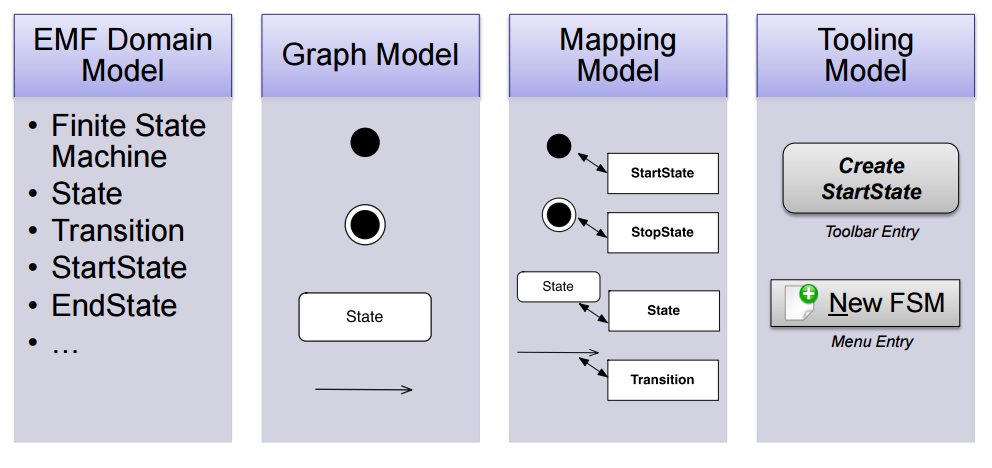
\includegraphics[width=.7\textwidth]{images/TableGMFSteps.PNG}
      \captionof{figure}{Models needed to create a graphical editor with GMF for the Finite State Machine example.}
      \label{mapmodel}
    \end{figure}
    
\section{Summary}\label{sec:summary}
Domain-specific modeling languages allow end-users with few or no programming skills 
to implement their own models, using languages they well understand. 
They can help to  avoid errors originating from biases in personal perception 
and issues in communication of requirements between different stakeholders in the development process (e.g. end-user, project-leaders, analysts, developers). 
There are different domain specific modeling languages providing support for creating valid models that
offering features to reduce  barriers (e.g. puzzle-piece shapes, soft-fail, auto-completion for text), which 
end-users  may have in implementing their own models. Additionally tools like Xtext and GMF offer support for creating new domain-specific modeling languages 
without requiring deep knowledge in compiler construction or programming a graphical model editor in a general purpose programming language.
Future research projects may use these tools and approaches to new domain-specific modeling languages to enable 
end-users to implement their own models and learn new scientific ideas in the process.
% 
% ---- Bibliography ----
% 
%\nocite{*}

%\bibliographystyle{splncs}
%\bibliography{citations}
\printbibliography
\end{document}

